\documentclass[11pt, a4paper]{article}
\usepackage[margin=2.4cm]{geometry}
\usepackage[T1]{fontenc}
\usepackage{lmodern}          % fontes vetoriais Type 1
\usepackage{cmap}             % ToUnicode CMap -> texto e acentos copiaveis
\usepackage[utf8]{inputenc}
\usepackage[brazil]{babel}
\usepackage{amsmath, amssymb, amsthm}
\usepackage{bm}
\usepackage{mathtools}
\usepackage{enumitem}
\usepackage{booktabs}
\usepackage{array}
\usepackage{xcolor}
\usepackage{titlesec}
\usepackage{parskip}
\usepackage{hyperref}
\usepackage{fancyhdr}
\usepackage{tcolorbox}
\usepackage{graphicx}
\tcbuselibrary{skins, breakable}

\definecolor{darkblue}{RGB}{15,55,115}
\definecolor{midblue}{RGB}{30,100,180}
\definecolor{theorybg}{RGB}{245,250,255}
\definecolor{questionbg}{RGB}{255,252,240}
\definecolor{evencolor}{RGB}{60,0,100}
\definecolor{rubricbg}{RGB}{248,246,252}
\definecolor{planbg}{RGB}{246,252,247}
\definecolor{plancolor}{RGB}{20,95,55}
\definecolor{trapbg}{RGB}{255,247,245}
\definecolor{trapcolor}{RGB}{150,35,35}

\hypersetup{colorlinks=true, linkcolor=darkblue, urlcolor=midblue,
  pdftitle={Resolucao --- Lista de Exercicios 4 --- Macroeconomia I MPE Insper},
  pdfauthor={Macroeconomia I --- MPE Insper 2026/T3}}

\setlength{\headheight}{14pt}
\pagestyle{fancy}
\fancyhf{}
\renewcommand{\headrulewidth}{0.4pt}
\fancyhead[L]{\small\textcolor{darkblue}{\textit{Macroeconomia I --- MPE Insper --- 2026/T3}}}
\fancyhead[R]{\small\textcolor{darkblue}{\thepage}}
\fancyfoot[C]{\small\textcolor{gray}{Resolução --- Lista de Exercícios 4}}

\titleformat{\section}[block]
  {\large\bfseries\color{darkblue}}{}{0pt}{}
  [\vspace{2pt}\color{darkblue}\rule{\textwidth}{1.5pt}\vspace{4pt}]

\tcbset{
  theorybox/.style={
    enhanced, breakable, colback=theorybg, colframe=darkblue,
    fonttitle=\bfseries\small, coltitle=white, boxrule=0.5pt, arc=3pt,
    left=6pt, right=6pt, top=4pt, bottom=4pt,
  },
  questionbox/.style={
    enhanced, breakable, colback=questionbg, colframe=gray!60,
    fonttitle=\bfseries\small, coltitle=black, boxrule=0.4pt, arc=2pt,
    left=6pt, right=6pt, top=4pt, bottom=4pt, title={\textit{Enunciado (original, em inglês)}},
  },
  rubricbox/.style={
    enhanced, breakable, colback=rubricbg, colframe=evencolor!70,
    fonttitle=\bfseries\small, coltitle=white, boxrule=0.4pt, arc=2pt,
    left=6pt, right=6pt, top=4pt, bottom=4pt, title={Onde estão os pontos},
  },
  planbox/.style={
    enhanced, breakable, colback=planbg, colframe=plancolor,
    fonttitle=\bfseries\small, coltitle=white, boxrule=0.5pt, arc=3pt,
    left=6pt, right=6pt, top=4pt, bottom=4pt,
  },
  trapbox/.style={
    enhanced, breakable, colback=trapbg, colframe=trapcolor!75,
    fonttitle=\bfseries\small, coltitle=white, boxrule=0.4pt, arc=2pt,
    left=6pt, right=6pt, top=4pt, bottom=4pt,
  },
}

\newcommand{\passo}[1]{\medskip\noindent\textbf{#1}\par\nobreak}
\newcommand{\intuicao}[1]{%
  \medskip\noindent\textcolor{midblue}{\textbf{Intuição econômica.}} #1\par}
\newcommand{\refbib}[1]{%
  \medskip\noindent{\small\textcolor{gray!60!black}{\textbf{Ref:} #1}}\par}
\newcommand{\resp}[1]{%
  \ifmmode {\color{darkblue}#1}\else\textcolor{darkblue}{\textbf{#1}}\fi}
\newcommand{\stst}{^{\ast}}
\newcommand{\wt}{\widetilde{w}}

\setlist[enumerate,1]{label=(\alph*), itemsep=6pt, parsep=2pt, leftmargin=1.6em}
\setlist[itemize,1]{itemsep=3pt, parsep=1pt, leftmargin=1.3em, topsep=3pt}

\begin{document}

%======================================================================
\begin{center}
{\LARGE\bfseries\color{darkblue} Resolução --- Lista de Exercícios 4\par}
\vspace{4pt}
{\large MACROECONOMIA 1 --- MPE Insper --- Prof.\ Pedro G.\ Duarte\par}
\vspace{2pt}
{\normalsize 2026, 3\textordmasculine{} trimestre \quad$\cdot$\quad Entrega: 31/08/2026\par}
\vspace{2pt}
{\small Trabalho e Lazer --- Kurlat (2020), cap.\ 7\par}
\end{center}
\vspace{6pt}

\begin{tcolorbox}[theorybox, title={Como ler este documento}]
\small
Duas questões, \textbf{dois modelos diferentes} --- é a primeira lista do trimestre em que
isso acontece. A Questão 1 é a escolha \emph{estática} consumo-lazer: a mesma máquina de
otimização da Aula 4, com lazer no lugar do consumo futuro. A Questão 2 é o modelo de
busca \textbf{DMP}, que não é uma escolha de otimização nenhuma --- é uma \emph{contabilidade
de fluxos} entre estoques, e tudo o que ela pede sai de duas linhas de álgebra.

\smallskip
O fio que liga as duas: em ambas, o resultado central é que \textbf{um preço deixa de
alocar corretamente}. Na Questão 1 o imposto abre uma cunha entre o que a firma paga e o
que o trabalhador recebe; na Questão 2 a firma que posta uma vaga não paga pelos efeitos
que impõe às outras. Nos dois casos o equilíbrio descentralizado não é o eficiente.

\smallskip
\textbf{Antes das resoluções vem o \hyperref[sec:plano]{Plano de leitura e preparo}}
(pp.\ \pageref{sec:plano}--\pageref{sec:fimplano}): item a item, o que ler no Kurlat, qual
ferramenta técnica o item cobra, qual é a armadilha e como saber que você já está pronto.
Se você ainda não tentou a lista, \textbf{leia só essa parte} e volte depois.

\smallskip
As respostas em destaque estão em \resp{azul}. As caixas
\textcolor{trapcolor}{\textbf{vermelhas}} são armadilhas; as
\textcolor{plancolor}{\textbf{verdes}}, preparo e método.
\end{tcolorbox}

\begin{center}
\small
\begin{tabular}{@{}lcl@{}}
\toprule
\textbf{Questão} & \textbf{Pontos} & \textbf{Base no Kurlat} \\
\midrule
1 --- Oferta de trabalho com imposto & 4 & Ex.\ \textbf{7.5} \emph{Prescott's Calculation}, itens (a)--(c) e (j)--(l) \\
2 --- Modelo de busca DMP & 6 & Ex.\ \textbf{7.7} \emph{The Beveridge Curve}, expandido; §7.5 \\
\bottomrule
\end{tabular}\\[3pt]
{\footnotesize A Questão 1 do enunciado é o Exercício 7.5 do livro com o lazer generalizado
de $\alpha\log(l)$ para $b\,l^{1-\gamma}/(1-\gamma)$. A Questão 2 converte o Exercício 7.7,
que no livro é \emph{estático} (desemprego ``antes'' e ``depois'' da contratação), em um
modelo \emph{dinâmico} com lei de movimento e estado estacionário.}
\end{center}

%======================================================================
\section[Plano de leitura e preparo]{Plano de leitura e preparo}
\label{sec:plano}
%======================================================================

\begin{tcolorbox}[planbox, title={A tese da lista, em uma frase}]
\small
\textbf{Quem responde a preço não é quem paga o preço} --- e as duas questões mostram isso
de dois jeitos: na Questão 1 o imposto muda o preço do lazer, mas o efeito sobre as horas
depende inteiramente de \emph{o que o governo faz com a receita}; na Questão 2 o preço que
guia a firma (a probabilidade $q$ de preencher a vaga) não incorpora nem o ganho que ela dá
aos desempregados nem o custo que impõe às outras firmas.
\end{tcolorbox}

\subsection*{1. O caminho mínimo de leitura ($\sim$2h30, antes de escrever qualquer coisa)}

\begin{center}
\small
\begin{tabular}{clp{7.4cm}c}
\toprule
\textbf{\#} & \textbf{Fonte} & \textbf{Por que} & \textbf{Tempo} \\
\midrule
1 & Kurlat §7.2, pp.\ 131--137
  & A escolha consumo-lazer, a restrição de tempo cheio e a decomposição renda
    $\times$ substituição (Fig.\ 7.2.2). É a espinha da Questão 1 inteira. & 35 min \\
2 & Kurlat, Exercício \textbf{7.5}, pp.\ 148--149
  & \textbf{É a Questão 1.} Os itens (a)--(c) do livro são o item (a) da lista; os itens
    (j)--(l), sobre a elasticidade de Frisch, são a parte ``discuta as propriedades''. & 25 min \\
3 & Kurlat §7.3, pp.\ 137--140
  & As evidências de elasticidade. Sem elas você não sabe dizer se a resposta que
    encontrou é grande ou pequena --- e é isso que o item (b) pede. & 20 min \\
4 & Kurlat §7.1, pp.\ 127--131
  & Estoques e fluxos do mercado de trabalho, $E$, $U$, vagas, a Beveridge empírica
    (Fig.\ 7.1.4). A Questão 2 é essa figura, derivada. & 25 min \\
5 & Kurlat §7.5, pp.\ 142--146
  & O modelo DMP: função de \emph{matching}, condição de postagem de vagas, e a
    discussão da Beveridge na p.\ 145. & 30 min \\
6 & Kurlat, Exercício \textbf{7.7}, p.\ 150
  & A Questão 2. Ler o original mostra o que o professor mudou: o livro é estático, a
    lista pede \textbf{estado estacionário}. Note a diferença de notação. & 15 min \\
\bottomrule
\end{tabular}
\end{center}

\passo{Complementares --- use só para intuição, nunca para elevar o nível técnico.}
Jones (2020), cap.\ 7, tem a versão gráfica do mercado de trabalho e uma boa exposição do
desemprego como fenômeno de fluxo. Romer (2012, arquivo local), cap.\ 11, traz o DMP
completo com barganha de Nash --- \textbf{muito além do que a lista pede}; use no máximo
para conferir a intuição das externalidades do item 2(d).

\subsection*{2. Item a item: o que ler, o que treinar, onde se erra}

\begin{center}
\footnotesize
\renewcommand{\arraystretch}{1.25}
\begin{tabular}{@{}p{0.8cm}p{2.35cm}p{3.85cm}p{3.95cm}p{3.35cm}@{}}
\toprule
\textbf{Item} & \textbf{Ler antes} & \textbf{Ferramenta que o item cobra} &
\textbf{Armadilha que custa ponto} & \textbf{Você está pronto quando} \\
\midrule

\textbf{1(a)} & §7.2, pp.\ 131--137; Ex.\ 7.5(a)--(b)
& Lagrangiano de dois bens; TMS $=$ preço relativo; substituir a restrição para obter
  \emph{uma} equação em $l$.
& Escrever a restrição como $c = wn$ e perder a dotação de tempo; esquecer que o preço do
  lazer é $(1-\tau)w$ e não $w$; parar antes de discutir as propriedades.
& Você escreve a restrição de tempo cheio e a CPO de memória, e sabe dizer por que a
  oferta é vertical quando $T=0$. \\

\textbf{1(b)} & §7.2, pp.\ 134--137 (renda $\times$ substituição); Ex.\ 7.5(c)
& Diferenciar a equação implícita; decompor o efeito; identificar o \emph{pivô} da
  rotação da reta.
& Dizer ``imposto reduz oferta'' sem condicionar em $T$ --- com $T=0$ o efeito é
  \textbf{exatamente zero}; confundir $T$ paramétrico com $T$ endógeno de orçamento
  equilibrado.
& Você responde ``depende de $T$'' \emph{antes} de fazer qualquer conta, e sabe desenhar
  a rotação em torno de $(\bar h,T)$. \\

\textbf{2(a)} & §7.1, pp.\ 127--131; §7.5, eq.\ (7.5.2)
& Contabilidade de estoques e fluxos: entra o que é contratado, sai o que é separado.
& Escrever $E_{t+1}$ com $sE_{t+1}$ em vez de $sE_t$; esquecer que $U_t = L-E_t$ torna a
  equação autônoma; descrever $\mu$ como ``produtividade'' sem dizer \emph{de quê}.
& Você escreve a lei de movimento sem hesitar e diz em uma frase o que $\mu$ mede. \\

\textbf{2(b)} & §7.5, pp.\ 142--146; Ex.\ 7.7
& Impor $E_{t+1}=E_t$; passar de níveis para taxas; isolar $v$; assinar a derivada.
& Impor estado estacionário e esquecer de dividir por $L$; dizer que a curva é
  decrescente ``porque os dados mostram'' em vez de derivar; não explicar \emph{as duas}
  forças que a inclinam.
& Você deriva $v(u)$ em três linhas e explica o sinal sem olhar o gráfico. \\

\textbf{2(c)} & §7.5, definição de \emph{matching}
& Usar retornos constantes de escala para colapsar $m(V,U)$ em função só de $\theta$.
& Não perceber que $\alpha+(1-\alpha)=1$ é o que faz tudo funcionar; errar o expoente de
  $q$ (é $\alpha-1$, negativo); provar $f=\theta q$ ``por substituição'' sem notar que é
  uma identidade contábil.
& Você deduz $f=\theta q$ em uma linha, direto das definições. \\

\textbf{2(d)} & §7.5, condição de postagem (7.5.1)
& Comparar produto \textbf{marginal} e produto \textbf{médio} de uma vaga; identificar
  quem ganha e quem perde.
& Responder só ``$f$ sobe e $q$ cai'' e parar --- a pergunta é sobre \emph{externalidade};
  dizer que a firma internaliza porque ``ela também sofre com $q$ menor''.
& Você explica por que $\partial m/\partial V=\alpha q$ é menor que o $q$ que a firma
  espera embolsar. \\

\textbf{2(e)} & §7.5, p.\ 145; Ex.\ 7.7(a)
& Distinguir mudança de parâmetro (desloca) de mudança de variável endógena (move ao
  longo).
& Tratar a queda de $\mu$ como movimento ao longo; dizer ``a curva desloca'' sem dizer
  \emph{para onde} e \emph{em que eixo}; esquecer que $s$ desloca no mesmo sentido.
& Você diz, sem desenhar, que a curva vai \textbf{para fora} e que a elasticidade é
  $-1/\alpha$. \\
\bottomrule
\end{tabular}
\end{center}

\subsection*{3. Cronograma sugerido --- três sessões}

\begin{center}
\small
\begin{tabular}{@{}llp{9.2cm}@{}}
\toprule
\textbf{Sessão} & \textbf{Duração} & \textbf{O que fazer} \\
\midrule
\textbf{I --- A escolha estática}
& $\sim$2h
& Leituras 1--3. Ao final, feche o livro e derive a CPO $bc\,l^{-\gamma}=(1-\tau)w$ do
  zero. Só depois faça \textbf{1(a)} e \textbf{1(b)}. Faça o caso $\gamma=1$ primeiro,
  com número, e só então generalize --- é muito mais rápido nessa ordem. \\
\textbf{II --- Os fluxos}
& $\sim$2h
& Leituras 4--6. Faça \textbf{2(a)}, \textbf{2(b)} e \textbf{2(c)} em sequência: são a
  mesma equação escrita de três formas. Desenhe a curva de Beveridge grande, à mão, com
  os eixos rotulados, antes de derivar qualquer coisa. \\
\textbf{III --- As duas conclusões}
& $\sim$1h30
& Faça \textbf{2(d)} e \textbf{2(e)}. Ao terminar, responda em voz alta: \emph{por que a
  firma não internaliza?} e \emph{qual é a diferença entre a curva se mover e a economia
  se mover sobre ela?} Se travar em qualquer uma, o problema está em 2(c), não aqui. \\
\bottomrule
\end{tabular}
\end{center}

\begin{tcolorbox}[trapbox, title={As cinco confusões que mais custam nota nesta lista}]
\small
\begin{enumerate}[label=\arabic*.]
\item \textbf{``Imposto sobre salário reduz a oferta de trabalho''.} Não necessariamente.
Com $\ln(c)$ e $T=0$, o efeito é \textbf{exatamente zero} --- para qualquer $\gamma$. O
sinal depende do que o governo faz com a receita, não da alíquota.
\item \textbf{$T$ paramétrico contra $T$ endógeno.} Com $T$ fixo, $\tau\uparrow$ empobrece
o domicílio e o efeito renda atenua a queda das horas. Com $T=\tau w n$ devolvido, o efeito
renda \emph{desaparece} e sobra só substituição. São respostas diferentes, e o enunciado
pede a primeira.
\item \textbf{$\gamma$ contra $1/\gamma$.} $\gamma$ é a curvatura da utilidade do lazer;
$1/\gamma$ é o que multiplica a elasticidade de Frisch. Trocar os dois inverte a
comparação com as estimativas empíricas.
\item \textbf{$s E_{t+1}$ em vez de $s E_t$.} A separação incide sobre quem \emph{estava}
empregado. Escrever a lei de movimento com o índice errado muda o estado estacionário.
\item \textbf{Deslocamento contra movimento.} $\theta$ é endógeno: move a economia
\emph{ao longo} da Beveridge. $\mu$ e $s$ são parâmetros: \emph{deslocam} a curva. Trocar
os dois é o erro mais caro do item 2(e).
\end{enumerate}
\end{tcolorbox}

\begin{tcolorbox}[planbox, title={O que você precisa saber de cor ao entrar na prova}]
\small
Sete objetos, três da Questão 1 e quatro da Questão 2. Nada mais desta lista é decorável.
\begin{align*}
\text{\textbf{1. Tempo cheio:}}\quad & c + \wt\,\ell = \wt\,\bar h + T,
  \qquad \wt \equiv (1-\tau)w \\[2pt]
\text{\textbf{2. CPO:}}\quad & \mathrm{TMS} = \frac{U_\ell}{U_c} = b\,c\,\ell^{-\gamma} = \wt \\[2pt]
\text{\textbf{3. Oferta implícita:}}\quad & \ell^{\gamma} + b\,\ell
  = b\,\bar h + \frac{b\,T}{\wt}
  \quad\Longrightarrow\quad n = \bar h - \ell \\[4pt]
\text{\textbf{4. Taxas:}}\quad & f = \mu\theta^{\alpha}, \qquad q = \mu\theta^{\alpha-1},
  \qquad f = \theta q \\[2pt]
\text{\textbf{5. Estado estacionário:}}\quad & s(1-u) = \mu v^{\alpha}u^{1-\alpha} = f\,u
  \quad\Longrightarrow\quad u\stst = \frac{s}{s+f} \\[2pt]
\text{\textbf{6. Beveridge:}}\quad & v = \left[\frac{s(1-u)}{\mu}\right]^{1/\alpha}
  u^{-\frac{1-\alpha}{\alpha}} \\[2pt]
\text{\textbf{7. Geometria:}}\quad & \text{o imposto \textbf{gira} a reta em torno de }
  (\bar h, T);\\
  & \theta \text{ \textbf{move ao longo} da Beveridge;\ } \mu \text{ e } s
  \text{ a \textbf{deslocam}.}
\end{align*}
De 3 saem 1(a) e 1(b); de 4 e 5 saem 2(b), 2(c) e 2(d); de 6 e 7 sai 2(e).
\end{tcolorbox}
\label{sec:fimplano}

%======================================================================
\section[Notação]{Notação}
\label{sec:notacao}
%======================================================================

O enunciado não fixa a dotação de tempo nem o símbolo das horas. Adoto a convenção do
Kurlat §7.2 e a declaro aqui, uma vez, para o documento inteiro.

\begin{center}
\small
\begin{tabular}{@{}cp{12.6cm}@{}}
\toprule
$\bar h$ & dotação de tempo. O Kurlat normaliza $\bar h = 1$; mantenho a letra para
  deixar visível onde ela entra. \\
$\ell$ & lazer, $\ell \in (0,\bar h]$ \\
$n \equiv \bar h - \ell$ & horas trabalhadas --- é a \emph{oferta de trabalho} do
  enunciado \\
$\wt \equiv (1-\tau)w$ & salário líquido. É o \textbf{preço do lazer}, e o único
  lugar por onde $\tau$ entra na decisão. \\
$M \equiv \wt\,\bar h + T$ & renda de tempo cheio (\emph{full income}): o que o domicílio
  teria se vendesse todo o seu tempo \\
\bottomrule
\end{tabular}
\end{center}

\passo{Um alerta sobre $\gamma=1$.} A função $b\,\ell^{1-\gamma}/(1-\gamma)$ não está
definida em $\gamma = 1$, mas o limite existe e vale $b\ln \ell$ a menos de uma constante.
Todas as fórmulas abaixo valem no limite; o caso $\gamma=1$ é justamente o do Kurlat,
Ex.\ 7.5, e é onde a lista fica com forma fechada.

%======================================================================
\section[Questão 1 --- oferta de trabalho com imposto]{Questão 1 --- Oferta de trabalho estática com imposto e transferência \small(4 pontos)}
%======================================================================

\begin{tcolorbox}[questionbox]
\small
Consider the static problem of a representative household choosing consumption and labor to
maximize the following utility function:
\[ U = \ln(c) + b\,\frac{(l)^{1-\gamma}}{1-\gamma} \tag{1} \]
where $c$ is consumption, $l$ is leisure, and parameters $b,\gamma > 0$. The household pays
a fraction $\tau$ of its wages as taxes and receives a lump-sum transfer from the government
of $T$.
\begin{enumerate}
\item Derive the labor supply equation for the household, characterize it graphically, and
  discuss its properties.
\item What is the effect of an increase in $\tau$ on labor supply? Show the result
  mathematically and graphically, and discuss the intuition behind it.
\end{enumerate}
\end{tcolorbox}

\subsection*{Item (a) --- a equação de oferta de trabalho}

\passo{Passo 1. Montar a restrição orçamentária.}
O domicílio vende $n = \bar h - \ell$ horas ao salário bruto $w$, paga a fração $\tau$ dos
salários em imposto e recebe $T$:
\[
c = (1-\tau)\,w\,(\bar h - \ell) + T = \wt\,(\bar h-\ell) + T .
\]
Passando $\wt \ell$ para a esquerda obtém-se a forma que interessa, a
\textbf{restrição de tempo cheio}:
\[
\boxed{\;c + \wt\,\ell \;=\; \underbrace{\wt\,\bar h + T}_{\displaystyle M}\;}
\tag{1.1}
\]

\intuicao{Escrita assim, a decisão vira uma escolha ordinária entre dois bens, $c$ e
$\ell$, com preços $1$ e $\wt$. O salário líquido \textbf{é o preço do lazer}: uma hora de
descanso custa $\wt$ unidades de consumo. Toda a Questão 1 é ler consequências dessa
frase. Note também onde $\tau$ e $T$ entram: $\tau$ mexe no \emph{preço relativo}; $T$
mexe só na \emph{renda}. É essa assimetria que produz a resposta do item (b).}

\passo{Passo 2. Condições de primeira ordem.}
Com $\lambda$ o multiplicador de (1.1),
\[
\mathcal{L} = \ln c + b\,\frac{\ell^{1-\gamma}}{1-\gamma}
  + \lambda\left[\wt\,\bar h + T - c - \wt\,\ell\right],
\]
\[
\frac{\partial\mathcal{L}}{\partial c} = \frac{1}{c} - \lambda = 0,
\qquad
\frac{\partial\mathcal{L}}{\partial \ell} = b\,\ell^{-\gamma} - \lambda\wt = 0 .
\]
Dividindo a segunda pela primeira elimina-se $\lambda$ e sobra a
\textbf{condição intratemporal}:
\[
\boxed{\;\mathrm{TMS} \;=\; \frac{U_\ell}{U_c}
 \;=\; \frac{b\,\ell^{-\gamma}}{1/c} \;=\; b\,c\,\ell^{-\gamma} \;=\; \wt\;}
\tag{1.2}
\]

A taxa marginal de substituição entre lazer e consumo iguala o salário líquido. É a mesma
estrutura da equação de Euler da Aula 4 --- lá o preço relativo era $1/[\beta(1+r)]$, aqui é
$\wt$ --- e é o único lugar em que $\tau$ aparece na decisão do domicílio.

\passo{Passo 3. Eliminar $c$ e obter a oferta de trabalho.}
De (1.2), $c = \wt\,\ell^{\gamma}/b$. Substituindo em (1.1):
\[
\frac{\wt\,\ell^{\gamma}}{b} + \wt\,\ell = \wt\,\bar h + T .
\]
Multiplicando tudo por $b/\wt$ (positivo, então o sinal não muda):
\[
\boxed{\;\Phi(\ell) \;\equiv\; \ell^{\gamma} + b\,\ell
 \;=\; b\,\bar h + \frac{b\,T}{\wt}
 \;=\; b\,\bar h + \frac{b\,T}{(1-\tau)w}\;}
\tag{1.3}
\]
e a oferta de trabalho é
\[
\resp{n\stst = \bar h - \ell\stst,
\qquad \ell\stst = \Phi^{-1}\!\left(b\,\bar h + \frac{b\,T}{(1-\tau)w}\right).}
\tag{1.4}
\]

\passo{Passo 4. A solução existe e é única.}
$\Phi'(\ell) = \gamma\ell^{\gamma-1} + b > 0$ para todo $\ell>0$: $\Phi$ é estritamente
crescente, logo $\Phi^{-1}$ está bem definida e (1.3) tem \textbf{no máximo uma} raiz.
A concavidade também é direta: substituindo a restrição na utilidade,
\[
\widetilde U(\ell) = \ln\!\big[\wt(\bar h - \ell) + T\big] + b\,\frac{\ell^{1-\gamma}}{1-\gamma},
\qquad
\widetilde U''(\ell) = -\frac{\wt^{\,2}}{[\wt(\bar h-\ell)+T]^{2}} - b\gamma\,\ell^{-\gamma-1} < 0 ,
\]
então o problema é estritamente côncavo e a CPO é suficiente. Como
$\widetilde U'(\ell)\to+\infty$ quando $\ell\to 0^{+}$, \textbf{nunca se escolhe lazer
zero}. O único canto possível é $\ell = \bar h$ (não participar), tratado adiante.

\begin{tcolorbox}[theorybox, title={Resposta do item (a)}]
\small
A oferta de trabalho é definida \textbf{implicitamente} por
\[
\ell^{\gamma} + b\,\ell = b\,\bar h + \frac{b\,T}{(1-\tau)w},
\qquad n = \bar h - \ell .
\]
Não há forma fechada para $\gamma$ arbitrário --- e não é preciso: $\Phi$ é estritamente
crescente, então $\ell$ está unicamente determinado e toda a estática comparativa sai de
diferenciar (1.3). Dois casos particulares \emph{têm} forma fechada e são os que
carregam a intuição:
\[
\resp{\gamma = 1:\quad \ell\stst = \frac{b}{1+b}\left(\bar h + \frac{T}{\wt}\right),
\qquad
n\stst = \frac{\bar h}{1+b} - \frac{b}{1+b}\cdot\frac{T}{\wt}}
\]
\[
\resp{T = 0,\ \text{qualquer }\gamma:\quad \ell^{\gamma} + b\,\ell = b\,\bar h
\ \Longrightarrow\ \ell\stst \text{ e } n\stst \text{ \textbf{não dependem de} } \wt .}
\]
\end{tcolorbox}

\subsubsection*{As propriedades --- é aqui que o item se ganha ou se perde}

\passo{Propriedade 1 (a mais importante). Com $T=0$ a oferta é \emph{vertical}.}
Olhe o lado direito de (1.3): se $T=0$, o salário líquido \textbf{some da equação}. Logo
$\ell\stst$ e $n\stst$ independem de $w$ e de $\tau$. A demonstração mais limpa não usa a
CPO: com $T=0$, a utilidade indireta é
\[
\widetilde U(\ell) = \ln\!\big[\wt(\bar h-\ell)\big] + b\,\frac{\ell^{1-\gamma}}{1-\gamma}
= \underbrace{\ln \wt}_{\text{constante em }\ell} + \ln(\bar h-\ell)
  + b\,\frac{\ell^{1-\gamma}}{1-\gamma},
\]
e o salário entra \textbf{aditivamente}: desloca o nível da utilidade, não o
$\arg\max$. A elasticidade (marshalliana) da oferta é exatamente zero.

\intuicao{Os dois efeitos se cancelam \emph{exatamente}. Um salário líquido maior torna o
lazer mais caro (efeito substituição, empurra $n$ para cima) e torna o domicílio mais rico
(efeito renda, empurra $n$ para baixo, porque lazer é bem normal). Com utilidade
logarítmica no consumo e \emph{nenhuma} renda não-salarial, a renda de tempo cheio
$M = \wt\bar h$ é proporcional a $\wt$ --- e a proporcionalidade é precisamente o que faz
os dois efeitos terem a mesma magnitude. Note que isso vale \textbf{para qualquer
$\gamma$}: a curvatura da utilidade do lazer não tem nada a ver com o cancelamento. Quem
manda é o $\ln(c)$.}

\begin{tcolorbox}[trapbox, title={Por que essa propriedade não é um defeito do modelo}]
\small
Uma oferta vertical parece patológica, mas é exatamente a hipótese que o curso precisa. É
o caso compatível com \textbf{crescimento equilibrado}: o salário real subiu por um fator
de dez ou mais nos últimos 150 anos e as horas trabalhadas por pessoa ficaram
aproximadamente estáveis (Kurlat §7.1). Uma oferta com elasticidade positiva grande
preveria que hoje trabalhamos muito mais que em 1870; uma com elasticidade negativa
grande, muito menos. O caso $\ln(c)$ é o que reproduz o fato estilizado --- e é por isso
que ele aparece em toda a macro de crescimento.
\end{tcolorbox}

\passo{Propriedade 2. Com $T>0$ a oferta é crescente no salário.}
Diferencie (1.3) em relação a $\wt$:
\[
\big(\gamma\ell^{\gamma-1}+b\big)\frac{\partial \ell}{\partial \wt}
= -\frac{b\,T}{\wt^{\,2}}
\quad\Longrightarrow\quad
\frac{\partial \ell}{\partial \wt} = \frac{-b\,T}{\wt^{\,2}\big(\gamma\ell^{\gamma-1}+b\big)} \le 0,
\qquad
\frac{\partial n}{\partial \wt} \ge 0 ,
\tag{1.5}
\]
com igualdade \textbf{se e somente se} $T=0$. A elasticidade não compensada é
\[
\varepsilon \equiv \frac{\partial n}{\partial \wt}\cdot\frac{\wt}{n}
= \frac{\ell^{\gamma} - b\,n}{n\big(\gamma\ell^{\gamma-1}+b\big)} \ \ge 0,
\tag{1.6}
\]
onde usei $b\,c = \wt \ell^{\gamma}$ de (1.2) e $T = c - \wt n$. Quando $T=0$, (1.3) dá
$\ell^{\gamma} = b\,n$ e o numerador zera --- consistente com a Propriedade 1.

\intuicao{A transferência quebra o empate. Com $T>0$, a renda de tempo cheio
$M = \wt\bar h + T$ \emph{não} é proporcional a $\wt$: quando o salário sobe, $M$ sobe
menos que proporcionalmente, porque a parcela $T$ não acompanha. O efeito renda fica
enfraquecido, o efeito substituição sobra, e as horas sobem.}

\passo{Propriedade 3. Salário de reserva e margem extensiva.}
Há canto em $\ell = \bar h$ (não participar) quando $\widetilde U'(\bar h) \ge 0$, isto é,
quando $b\,\bar h^{-\gamma} \ge \wt/T$. Equivalentemente, participa-se se e somente se
\[
\resp{w > w^{r} \equiv \frac{b\,T\,\bar h^{-\gamma}}{1-\tau}} .
\tag{1.7}
\]
$w^r$ é a TMS avaliada no ponto de não trabalhar, $(c,\ell) = (T,\bar h)$. Duas leituras:
com $T=0$ o salário de reserva é \textbf{zero} e sempre se participa; e $\tau\uparrow$
\textbf{eleva} $w^r$, ou seja, o imposto também expulsa gente pela margem extensiva --- a
margem que, segundo o Kurlat §7.3, responde mais que a intensiva.

\passo{Propriedade 4. A elasticidade de Frisch e o papel de $\gamma$.}
$\gamma$ não afeta o \emph{sinal} de nada; ele governa a \emph{magnitude}. O jeito limpo
de ver isso é a elasticidade de Frisch --- a resposta das horas ao salário
\textbf{mantendo o consumo constante} (Kurlat, Ex.\ 7.5(j)--(l)). De (1.2) com $c$ fixo,
\[
\ell = \left(\frac{b\,c}{\wt}\right)^{1/\gamma}
\quad\Longrightarrow\quad
\resp{\varepsilon^{F} \;=\; \frac{\partial n}{\partial\wt}\cdot\frac{\wt}{n}\bigg|_{c}
 \;=\; \frac{1}{\gamma}\cdot\frac{\ell}{n}
 \;=\; \frac{\ell}{\gamma\,(\bar h-\ell)} } .
\tag{1.8}
\]
Então $\gamma$ é o \textbf{inverso} da substitutibilidade do lazer: $\gamma$ alto significa
utilidade do lazer muito curva, lazer que o domicílio quer suave, e oferta rígida. E note
o fator $\ell/n$: como se passa a maior parte do tempo fora do trabalho, a Frisch é
\emph{muito} maior que a marshalliana. Com os números de Prescott ($\gamma=1$,
$\ell=0{,}70$), $\varepsilon^F = 2{,}33$ contra $\varepsilon = 0{,}31$.

\passo{Caracterização gráfica.}
São dois planos, e os dois são cobrados.

\begin{center}
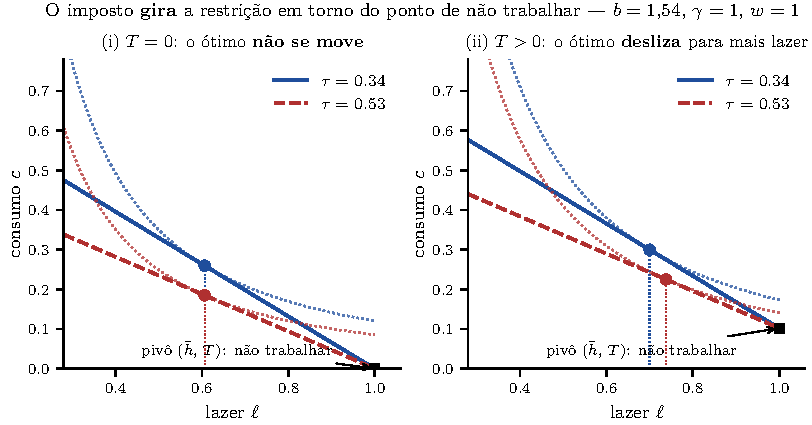
\includegraphics[width=\textwidth]{fig/fig_l4q1_lazer.pdf}
\end{center}

No plano $(\ell,c)$ a restrição (1.1) é uma reta de inclinação $-\wt$ que passa
\textbf{obrigatoriamente} pelo ponto $(\bar h,\,T)$: se o domicílio não trabalha, consome
exatamente a transferência, seja qual for o salário. Esse ponto é o \textbf{pivô} de
qualquer mudança em $w$ ou $\tau$. O ótimo é a tangência entre a reta e uma curva de
indiferença. No painel (i), com $T=0$, o pivô está sobre o eixo horizontal e a tangência
ocorre sempre no mesmo $\ell$; no painel (ii), com $T>0$, o pivô sobe e a tangência desliza.

\begin{center}
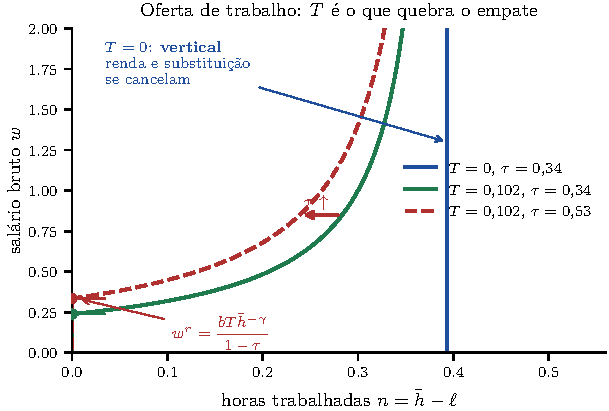
\includegraphics[width=0.78\textwidth]{fig/fig_l4q1_oferta.pdf}
\end{center}

No plano $(n,w)$ --- a curva de oferta propriamente dita --- o caso $T=0$ é uma
\textbf{reta vertical} em $n = \bar h/(1+b)$ (para $\gamma=1$); o caso $T>0$ é uma curva
crescente que \emph{parte} do salário de reserva $w^r$ e tende assintoticamente à vertical
quando $w\to\infty$, porque a importância relativa de $T$ desaparece. Um $\tau$ maior
desloca essa curva para a esquerda e eleva $w^r$.

\begin{tcolorbox}[rubricbox]
\small
Estimo 2,5 dos 4 pontos neste item.
\begin{itemize}
\item \textbf{0,8} --- restrição de tempo cheio correta, com $\wt=(1-\tau)w$ identificado
  como preço do lazer.
\item \textbf{0,7} --- CPO $b\,c\,\ell^{-\gamma}=\wt$ e a equação implícita (1.3).
\item \textbf{0,5} --- os dois gráficos, com o \textbf{pivô} $(\bar h,T)$ marcado. Sem o
  pivô, o gráfico não explica nada do item (b).
\item \textbf{0,5} --- as propriedades. O item diz ``discuss its properties'': listar a
  verticalidade com $T=0$, a monotonicidade com $T>0$ e o salário de reserva. Quem só
  resolve e para perde esses pontos.
\end{itemize}
\end{tcolorbox}

\refbib{Kurlat (2020), cap.\ 7, §7.2 (pp.\ 131--137) e Exercício 7.5(a)--(b) (p.\ 148).
Regras do projeto: \texttt{rules/05\_trabalho\_lazer.md}, seção ``Teoria estática''.}

\subsection*{Item (b) --- o efeito de um aumento de $\tau$}

\passo{Passo 1. Onde $\tau$ entra.}
Em (1.3), $\tau$ aparece \textbf{em um único lugar}: no termo $b\,T/[(1-\tau)w]$. Isso já
antecipa a resposta inteira: se $T=0$, o termo é nulo e $\tau$ não tem por onde agir.

\passo{Passo 2. A derivada.}
Diferenciando (1.3) em $\tau$, com $\partial\wt/\partial\tau = -w$:
\[
\big(\gamma\ell^{\gamma-1}+b\big)\frac{\partial \ell}{\partial\tau}
= b\,T\cdot\frac{\partial}{\partial\tau}\!\left[\frac{1}{(1-\tau)w}\right]
= \frac{b\,T}{w\,(1-\tau)^{2}} ,
\]
\[
\resp{\frac{\partial \ell}{\partial \tau}
 = \frac{b\,T}{w\,(1-\tau)^{2}\big(\gamma\ell^{\gamma-1}+b\big)} \ \ge 0,
\qquad
\frac{\partial n}{\partial \tau}
 = -\,\frac{b\,T}{w\,(1-\tau)^{2}\big(\gamma\ell^{\gamma-1}+b\big)} \ \le 0 ,}
\tag{1.9}
\]
\textbf{com igualdade se e somente se $T = 0$}. Em elasticidade,
$\dfrac{d\ln n}{d\tau} = -\dfrac{\varepsilon}{1-\tau}$, com $\varepsilon$ de (1.6).

\begin{tcolorbox}[theorybox, title={Resposta do item (b)}]
\small
\resp{Um aumento de $\tau$ nunca aumenta a oferta de trabalho, mas o efeito é
\textbf{exatamente zero} quando $T=0$ e estritamente negativo quando $T>0$.} O sinal não
depende de $b$ nem de $\gamma$ --- só da presença da transferência. $\gamma$ afeta apenas
a \emph{magnitude}, pelo denominador $\gamma\ell^{\gamma-1}+b$: quanto maior $\gamma$,
menor a resposta.
\end{tcolorbox}

\passo{Passo 3. A decomposição renda $\times$ substituição.}
\begin{center}
\small
\renewcommand{\arraystretch}{1.3}
\begin{tabular}{@{}lp{5.0cm}cc@{}}
\toprule
\textbf{Canal} & \textbf{Mecanismo} & \textbf{Sobre $\ell$} & \textbf{Sobre $n$} \\
\midrule
Substituição & $\wt\downarrow$ barateia o lazer & $\uparrow$ & $\downarrow$ \\
Renda & $\wt\downarrow$ empobrece; lazer é bem normal & $\downarrow$ & $\uparrow$ \\
\midrule
\textbf{Líquido, $T=0$} & renda de tempo cheio $M=\wt\bar h$ é \emph{proporcional} a
  $\wt$; com $\ln(c)$ os dois canais têm a mesma magnitude & $0$ & $\bm{0}$ \\
\textbf{Líquido, $T>0$} & $M=\wt\bar h + T$ cai \emph{menos} que proporcionalmente;
  o canal renda enfraquece & $\uparrow$ & $\bm{\downarrow}$ \\
\bottomrule
\end{tabular}
\end{center}

\intuicao{A pergunta ``o imposto reduz a oferta de trabalho?'' está mal posta enquanto não
se diz \textbf{o que acontece com a receita}. Se o dinheiro sai da economia ($T=0$), o
domicílio fica mais pobre \emph{na mesma proporção} em que o lazer fica mais barato, e com
$\ln(c)$ as duas forças se anulam. Se o dinheiro volta como transferência fixa ($T>0$), o
domicílio não fica tão mais pobre --- e aí o barateamento do lazer domina. O imposto
distorce \emph{porque} é devolvido, não apesar disso.}

\passo{Passo 4. O gráfico.}
Volte ao painel de $(\ell,c)$ da página anterior. Um $\tau$ maior reduz $\wt$ e portanto
\textbf{achata} a reta orçamentária --- mas ela \emph{gira em torno de $(\bar h,T)$}, que
não se move. É toda a resposta gráfica do item:
\begin{itemize}
\item \textbf{Painel (i), $T=0$:} o pivô está na origem do eixo do lazer. A reta gira em
torno de um ponto do próprio eixo, o que preserva a razão entre as duas ``pernas'' do
orçamento. Com preferências log no consumo a tangência fica \textbf{no mesmo $\ell$}.
\item \textbf{Painel (ii), $T>0$:} o pivô está \emph{acima} do eixo. A rotação em torno de
um ponto interno não é uma mudança proporcional de renda, e a tangência \textbf{desliza
para a direita}: mais lazer, menos horas.
\end{itemize}
No plano $(n,w)$, a curva de oferta se desloca para a esquerda e o salário de reserva sobe,
de $b T\bar h^{-\gamma}$ para $b T\bar h^{-\gamma}/(1-\tau)$.

\begin{tcolorbox}[planbox, title={Extensão que vale meio ponto: e se o governo devolver toda a receita?}]
\small
O enunciado trata $T$ como \textbf{parâmetro}, e é assim que o item deve ser resolvido. Mas
vale dizer uma frase sobre o fechamento natural, porque ele inverte a conclusão e é o que o
Kurlat faz no Ex.\ 7.5(e). Suponha orçamento equilibrado, $T = \tau\,w\,n$. O domicílio
\emph{continua} tomando $T$ como dado --- a CPO (1.2) não muda --- mas em equilíbrio
$c = \wt n + T = w\,n$. Substituindo em (1.2):
\[
b\,w\,(\bar h - \ell)\,\ell^{-\gamma} = (1-\tau)\,w
\quad\Longrightarrow\quad
\resp{(1-\tau)\,\ell^{\gamma} + b\,\ell = b\,\bar h},
\qquad
\gamma = 1:\ \resp{\ell = \frac{b}{\,b+1-\tau\,}} .
\]
Diferenciando, $\partial\ell/\partial\tau = \ell^{\gamma}/[(1-\tau)\gamma\ell^{\gamma-1}+b] > 0$:
agora $\partial n/\partial\tau < 0$ \textbf{sempre}, inclusive no caso log. O rebate
neutraliza o efeito renda e deixa o efeito substituição sozinho. \textbf{Moral:} o mesmo
imposto é neutro ou distorcivo conforme o destino da receita. Diga isso e o item (b) fica
completo.
\end{tcolorbox}

\passo{Passo 5. Quanto é isso, em números?}
O Kurlat calibra exatamente este modelo com $\gamma=1$ para comparar EUA e Europa
(Ex.\ 7.5(d)--(f)). Com $b = 1{,}54$, $w=1$, $\bar h = 1$:

\begin{center}
\small
\begin{tabular}{@{}lccccc@{}}
\toprule
& $\tau$ & $T$ & $\ell\stst$ & $n\stst$ & receita $\tau w n$ \\
\midrule
EUA & 0{,}34 & 0{,}102 & 0{,}7000 & \textbf{0{,}3000} & 0{,}1020 \\
Europa & 0{,}53 & 0{,}124 & 0{,}7663 & \textbf{0{,}2337} & 0{,}1239 \\
\bottomrule
\end{tabular}
\end{center}

Os dois orçamentos fecham (receita $=T$, a menos de arredondamento), então esta é a versão
de orçamento equilibrado. A Europa trabalha \resp{22{,}1\% menos} que os EUA, e com
$Y = L = n$ o PIB per capita europeu fica $22{,}1\%$ abaixo --- \textbf{inteiramente}
explicado pela diferença de alíquota. É o resultado célebre de Prescott.

\begin{tcolorbox}[trapbox, title={O que essa conta NÃO prova}]
\small
A conta só funciona porque a elasticidade de Frisch implícita é alta. Por (1.8), com
$\ell = 0{,}70$ e $\gamma=1$, $\varepsilon^F = 0{,}70/0{,}30 = \mathbf{2{,}33}$. As
estimativas microeconométricas ficam entre \textbf{0,4 e 1} (Kurlat, Ex.\ 7.5(l)). Com uma
elasticidade nessa faixa, o mesmo diferencial de imposto explicaria uma fração pequena do
hiato de horas, e o resto teria de vir de outra coisa --- instituições do mercado de
trabalho, sindicatos, regulação de jornada, preferências. Dizer ``o imposto explica o
hiato EUA--Europa'' sem essa ressalva é justamente o tipo de conclusão que o enunciado
pede que você discuta, não que repita.
\end{tcolorbox}

\begin{tcolorbox}[rubricbox]
\small
Estimo 1,5 dos 4 pontos neste item.
\begin{itemize}
\item \textbf{0,5} --- a derivada (1.9) com o sinal correto e a condição $T=0$ explicitada.
\item \textbf{0,4} --- o gráfico da rotação, com o pivô $(\bar h,T)$ identificado.
\item \textbf{0,6} --- a intuição: renda $\times$ substituição, e por que $T$ decide o
  empate. É o que o enunciado chama de ``the intuition behind it'', e é onde está a maior
  parte do julgamento.
\end{itemize}
\end{tcolorbox}

\refbib{Kurlat (2020), cap.\ 7, §7.2 (pp.\ 134--137, decomposição renda $\times$
substituição, Fig.\ 7.2.2) e Exercício 7.5(c)--(f), (j)--(l) (pp.\ 148--149).}

%======================================================================
\section[Questão 2 --- modelo de busca DMP]{Questão 2 --- O modelo de busca de Diamond, Mortensen e Pissarides \small(6 pontos)}
%======================================================================

\begin{tcolorbox}[questionbox]
\small
Consider the search model of Diamond, Mortensen and Pissarides (DMP). Let $U$ be the number
of unemployed workers, $V$ the number of vacancies posted by firms, and $E$ the number of
employed workers. The labor force $L = U+E$ is constant. The number of new matches formed
each period is given by the matching function
\[ m(V,U) = \mu V^{\alpha}U^{1-\alpha} \tag{2} \]
where $\alpha\in(0,1)$ and $\mu>0$. Each period, a fraction $s\in(0,1)$ of employed workers
loses their job exogenously. Define the unemployment rate $u\equiv U/L$, the vacancy rate
$v \equiv V/L$, and market tightness $\theta \equiv V/U$.
\begin{enumerate}
\item Write down the law of motion of employment, $E_{t+1}$, as a function of $E_t$, $V_t$
  and $U_t$. Explain what each term represents. What does the parameter $\mu$ measure, and
  how does a higher $\mu$ change the law of motion?
\item Impose steady state and derive the equation that equates job creation and job
  destruction. Use it to obtain the Beveridge curve of this economy. Draw it in $(u,v)$
  space and explain why it slopes the way it does.
\item Define the job finding rate $f\equiv m/U$ and the job filling rate $q\equiv m/V$.
  Write both as functions of $\theta$ alone. Show that $f=\theta q$, and say whether each
  rate rises or falls with $\theta$.
\item Suppose a single firm posts one extra vacancy. What happens to $f$ and to $q$? Which
  agents in the economy gain and which lose? Does the firm take these effects into account
  when it decides to post the vacancy?
\item What is the effect of a fall in $\mu$ on the Beveridge curve? What does this imply
  for the vacancy rate at a given unemployment rate? Explain how this differs from a
  movement along the curve.
\end{enumerate}
\end{tcolorbox}

\begin{tcolorbox}[theorybox, title={A mudança de chave em relação à Questão 1}]
\small
Aqui \textbf{não há problema de otimização}. Ninguém maximiza nada nesta questão. O que há
é contabilidade de estoques e fluxos: $E$ e $U$ são estoques, $sE$ e $m(V,U)$ são fluxos, e
todo o modelo é a afirmação de que o estoque de amanhã é o de hoje mais o que entra menos o
que sai. Se você começar montando um lagrangiano, está no caminho errado.

\smallskip
A recompensa dessa simplicidade: o desemprego deixa de ser um estoque a explicar e vira o
resultado de uma \textbf{razão entre fluxos}. Duas economias com o mesmo desemprego podem
ser completamente diferentes --- uma com muita rotatividade e desemprego curto, outra com
pouca rotatividade e desemprego longo. É a leitura que o Kurlat §7.1 faz dos dados dos EUA:
perda de emprego de 1\% a 2\% ao mês contra saída do desemprego de $\sim$30\% ao mês.
\end{tcolorbox}

\subsection*{Item (a) --- a lei de movimento do emprego}

\passo{A equação.}
O estoque de empregados no início de $t+1$ é o de $t$, menos os que foram separados, mais
os que foram contratados:
\[
\boxed{\;E_{t+1} \;=\; \underbrace{E_t}_{\text{estoque}}
 \;-\; \underbrace{s\,E_t}_{\text{destruição}}
 \;+\; \underbrace{m(V_t,U_t)}_{\text{criação}}
 \;=\; (1-s)\,E_t \;+\; \mu\,V_t^{\alpha}\,U_t^{1-\alpha}\;}
\tag{2.1}
\]

\passo{O que cada termo representa.}
\begin{itemize}
\item $(1-s)E_t$ --- os empregados que \textbf{sobrevivem} ao período. A separação é
  exógena e proporcional: $sE_t$ trabalhadores perdem o emprego, independentemente de
  quem sejam ou de qualquer decisão. É a \emph{destruição de empregos}.
\item $m(V_t,U_t) = \mu V_t^{\alpha}U_t^{1-\alpha}$ --- os encontros bem-sucedidos entre
  vagas e desempregados no período. É a \emph{criação de empregos}, e é a única parte do
  modelo em que a estrutura do mercado importa.
\item Como $L = U_t + E_t$ é constante, $U_t = L - E_t$, e (2.1) é uma equação de
  diferenças \textbf{autônoma} em $E_t$, dado $V_t$:
  $E_{t+1} = (1-s)E_t + \mu V_t^{\alpha}(L-E_t)^{1-\alpha}$.
\end{itemize}

Em taxas (dividindo por $L$, com $e \equiv E/L = 1-u$):
\[
e_{t+1} = (1-s)\,e_t + \mu\,v_t^{\alpha}\,u_t^{1-\alpha},
\qquad\text{ou}\qquad
u_{t+1} = u_t + s\,(1-u_t) - \mu\,v_t^{\alpha}\,u_t^{1-\alpha} .
\tag{2.2}
\]

\passo{O que $\mu$ mede.}
\resp{$\mu$ é a \textbf{eficiência do processo de encontro} --- a ``PTF da função de
\emph{matching}''.} Ela responde: dados um estoque de vagas e um estoque de procurantes,
quantos casamentos o mercado consegue produzir? Um $\mu$ maior significa menos atrito:
melhor informação sobre onde estão as vagas, menor descasamento geográfico ou de
qualificação, agências de emprego e plataformas mais eficazes, maior intensidade de busca.

Note que $m$ tem retornos constantes de escala, $\alpha + (1-\alpha) = 1$, então
$V^{\alpha}U^{1-\alpha}$ já tem unidade de ``trabalhadores'' e \textbf{$\mu$ é
adimensional} --- um puro escalar de eficiência. Esse detalhe é o que faz o item (c)
funcionar.

\passo{Efeito de um $\mu$ maior.}
$\mu$ multiplica \emph{apenas} o termo de criação. Para quaisquer $V_t$ e $U_t$ dados, a
criação sobe proporcionalmente: um $\mu$ 10\% maior produz 10\% mais contratações. Três
consequências:
\begin{enumerate}[label=(\roman*)]
\item o emprego cresce mais rápido a partir de qualquer ponto inicial;
\item a convergência ao estado estacionário é mais rápida;
\item o estado estacionário tem \textbf{menos desemprego} --- pelo item (b),
  $u\stst = s/(s+\mu\theta^{\alpha})$, decrescente em $\mu$.
\end{enumerate}
Graficamente, no plano $(e_t, e_{t+1})$, a curva $(1-s)e + \mu v^{\alpha}(1-e)^{1-\alpha}$
se desloca para cima e cruza a diagonal de $45^{\circ}$ mais à direita.

\begin{tcolorbox}[trapbox, title={Duas ressalvas de consistência}]
\small
\textbf{1.} O modelo só faz sentido enquanto $m \le \min\{U_t,\,V_t\}$ --- não se pode
criar mais empregos do que há desempregados ou vagas. Isso exige $f = \mu\theta^{\alpha}\le 1$
e $q = \mu\theta^{\alpha-1}\le 1$. Com a calibração mensal usual ($f\approx 0{,}30$,
$q\approx 0{,}43$) a restrição não morde, mas ela existe.

\smallskip
\textbf{2.} O índice temporal importa: é $sE_t$, não $sE_{t+1}$. A separação incide sobre
quem \emph{estava} empregado no início do período. Trocar isso muda o estado estacionário
para $u\stst = s/(s+f-sf)$ e derruba o item (b) inteiro.
\end{tcolorbox}

\begin{tcolorbox}[rubricbox]
\small
Estimo 1,0 dos 6 pontos. \textbf{0,4} pela equação (2.1) com os índices corretos;
\textbf{0,3} pela explicação dos dois termos como destruição e criação; \textbf{0,3} por
identificar $\mu$ como eficiência de \emph{matching} e dizer que ela escala só o termo de
criação. Quem chama $\mu$ de ``produtividade do trabalho'' perde os últimos 0,3.
\end{tcolorbox}

\refbib{Kurlat (2020), cap.\ 7, §7.5 (pp.\ 142--146), eq.\ (7.5.2); §7.1 (pp.\ 127--131)
para os fluxos medidos.}

\subsection*{Item (b) --- estado estacionário e a curva de Beveridge}

\passo{Passo 1. Impor estado estacionário.}
Em estado estacionário $E_{t+1} = E_t = E$. De (2.1):
\[
E = (1-s)E + m(V,U)
\quad\Longrightarrow\quad
\boxed{\;\underbrace{s\,E}_{\text{destruição}}
 \;=\; \underbrace{\mu\,V^{\alpha}U^{1-\alpha}}_{\text{criação}}\;}
\tag{2.3}
\]

\resp{Esta é a equação que iguala criação e destruição de empregos.} O desemprego é
constante não porque ninguém se move, mas porque \textbf{os dois fluxos se cancelam}: todo
mês $sE$ pessoas perdem o emprego e exatamente $m$ pessoas conseguem um.

\passo{Passo 2. Passar para taxas.}
Divida (2.3) por $L$. Como $E/L = 1-u$, $V/L = v$ e $U/L = u$, e $m$ tem retornos
constantes:
\[
\boxed{\;s\,(1-u) \;=\; \mu\,v^{\alpha}\,u^{1-\alpha}\;}
\tag{2.4}
\]

\passo{Passo 3. Isolar $v$ --- a curva de Beveridge.}
De (2.4),
\[
v^{\alpha} = \frac{s\,(1-u)}{\mu\,u^{1-\alpha}}
\quad\Longrightarrow\quad
\resp{v(u) \;=\; \left[\frac{s\,(1-u)}{\mu}\right]^{1/\alpha}
   u^{-\frac{1-\alpha}{\alpha}} } .
\tag{2.5}
\]

Este é o lugar geométrico dos pares $(u,v)$ compatíveis com desemprego constante --- a
\textbf{curva de Beveridge} do modelo.

\passo{Passo 4. A inclinação.}
Tome logaritmos de (2.5):
$\ln v = \frac{1}{\alpha}\big[\ln s - \ln\mu + \ln(1-u)\big] - \frac{1-\alpha}{\alpha}\ln u$.
Derivando,
\[
\frac{d\ln v}{d\ln u}
 = -\frac{1}{\alpha}\left[\frac{u}{1-u} + (1-\alpha)\right] < 0,
\qquad
\frac{dv}{du} = -\frac{v}{\alpha\,u}\left[\frac{u}{1-u} + 1-\alpha\right] < 0 .
\tag{2.6}
\]
Além de decrescente, a curva é \textbf{convexa}: $v\to\infty$ quando $u\to 0^{+}$ e
$v\to 0$ quando $u\to 1^{-}$. Na calibração da figura, $|dv/du|$ cai de $3{,}45$ em
$u=3\%$ para $0{,}31$ em $u=10\%$.

\begin{center}
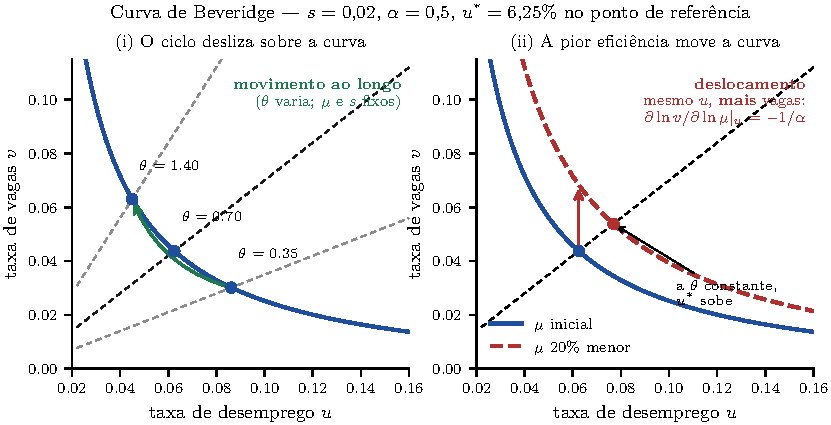
\includegraphics[width=\textwidth]{fig/fig_l4q2_beveridge.pdf}
\end{center}

\begin{tcolorbox}[theorybox, title={Por que a curva é negativamente inclinada --- duas forças, mesmo sentido}]
\small
Olhe (2.4) como um equilíbrio de fluxos e pergunte o que acontece quando $u$ sobe,
mantendo $v$ fixo.
\begin{enumerate}[label=\arabic*.]
\item \textbf{Lado esquerdo --- menos empregos a repor.} Se $u$ é maior, $1-u$ é menor:
há menos gente empregada e portanto \emph{menos separações} para compensar. A necessidade
de contratação cai.
\item \textbf{Lado direito --- cada vaga fica mais produtiva.} Com mais desempregados
procurando, o mesmo estoque de vagas gera mais encontros: $\mu v^{\alpha}u^{1-\alpha}$
sobe em $u$. A oferta de contratações sobe.
\end{enumerate}
A necessidade caiu e a capacidade subiu: \textbf{as duas forças pedem menos vagas}. Daí
$dv/du<0$. Note que isso é uma afirmação sobre o \emph{estado estacionário}, não sobre
causalidade --- a curva diz quais combinações são sustentáveis, não qual delas ocorre.
Determinar o ponto exige uma segunda relação, a condição de postagem de vagas do Kurlat
§7.5, que a lista não pede.
\end{tcolorbox}

\intuicao{A leitura empírica é imediata e é a Fig.\ 7.1.4 do Kurlat: em expansões as firmas
postam muitas vagas e o desemprego é baixo (canto superior esquerdo); em recessões o
oposto (canto inferior direito). Cada ponto do gráfico do livro é um mês da economia
americana, e a nuvem desce da esquerda para a direita exatamente como (2.5) prevê.}

\begin{tcolorbox}[rubricbox]
\small
Estimo 1,5 dos 6 pontos. \textbf{0,4} por impor $E_{t+1}=E_t$ e chegar a (2.3) nomeando
criação e destruição; \textbf{0,4} pela passagem a taxas e por isolar $v$ em (2.5);
\textbf{0,3} pelo gráfico com eixos corretos ($u$ na horizontal, $v$ na vertical);
\textbf{0,4} pela explicação da inclinação. Quem só diz ``é decrescente porque os dados
mostram'' fica com no máximo 0,1 desses últimos 0,4 --- o enunciado pede \emph{explain why
it slopes the way it does}, e a resposta tem de sair de (2.4).
\end{tcolorbox}

\subsection*{Item (c) --- as taxas $f$ e $q$ como funções de $\theta$}

\passo{Passo 1. As duas definições, e o único truque.}
O truque é sempre o mesmo: retornos constantes de escala permitem dividir dentro da função.
\[
f \equiv \frac{m}{U} = \frac{\mu V^{\alpha}U^{1-\alpha}}{U}
 = \mu\left(\frac{V}{U}\right)^{\alpha}
\quad\Longrightarrow\quad
\resp{f(\theta) = \mu\,\theta^{\alpha}} ,
\tag{2.7}
\]
\[
q \equiv \frac{m}{V} = \frac{\mu V^{\alpha}U^{1-\alpha}}{V}
 = \mu\left(\frac{U}{V}\right)^{1-\alpha}
\quad\Longrightarrow\quad
\resp{q(\theta) = \mu\,\theta^{\alpha-1} = \mu\,\theta^{-(1-\alpha)}} .
\tag{2.8}
\]

Ambas dependem \textbf{só} de $\theta$: os níveis de $V$ e $U$ são irrelevantes, apenas a
razão importa. É essa propriedade que torna o DMP tratável, e ela vem inteiramente do
$\alpha + (1-\alpha) = 1$ no expoente.

\passo{Passo 2. A identidade $f=\theta q$.}
Direto das definições, sem passar pela forma funcional:
\[
f = \frac{m}{U} = \frac{m}{V}\cdot\frac{V}{U} = q\,\theta .
\tag{2.9}
\]
Conferindo com (2.7)--(2.8): $\theta q = \theta\cdot\mu\theta^{\alpha-1} = \mu\theta^{\alpha} = f$.
\resp{$f=\theta q$ é uma identidade contábil}, não um resultado do modelo: o mesmo fluxo $m$
está sendo dividido ora pelo estoque de procurantes, ora pelo estoque de vagas.

\passo{Passo 3. Monotonicidade.}
\[
\frac{df}{d\theta} = \alpha\,\mu\,\theta^{\alpha-1} > 0,
\qquad
\frac{dq}{d\theta} = -(1-\alpha)\,\mu\,\theta^{\alpha-2} < 0 ,
\]
\[
\resp{\varepsilon_{f,\theta} = \alpha > 0, \qquad
      \varepsilon_{q,\theta} = -(1-\alpha) < 0, \qquad
      \varepsilon_{f,\theta} - \varepsilon_{q,\theta}\big|_{\text{sinal}}:\ \ \alpha + (1-\alpha) = 1 .}
\]
As duas elasticidades somam $1$ em valor absoluto --- é o reflexo de $f=\theta q$, que em
logs é $\ln f = \ln\theta + \ln q$.

\begin{center}
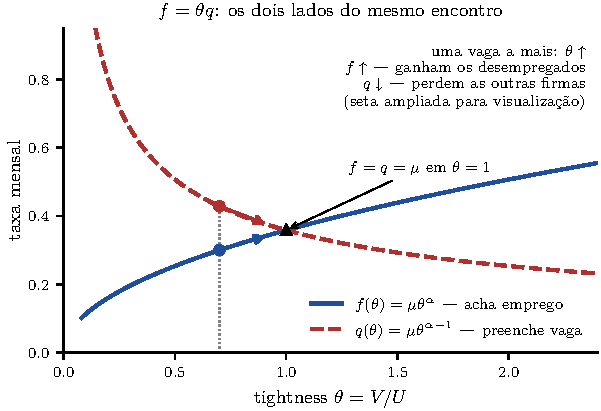
\includegraphics[width=0.78\textwidth]{fig/fig_l4q2_fq.pdf}
\end{center}

\intuicao{Um mercado ``apertado'' (\emph{tight}), com muitas vagas por desempregado, é
\textbf{bom para quem procura emprego e ruim para quem procura trabalhador}. $\theta$ é a
única variável que separa os dois lados, e ela os afeta em direções opostas. Em $\theta=1$
--- uma vaga por desempregado --- as duas taxas coincidem em $\mu$: é o único ponto em que
a facilidade é simétrica.}

\passo{Passo 4. O subproduto que vale ouro no item (e).}
Substituindo $f$ em (2.4): dividindo os dois lados por $u$,
$s\,\frac{1-u}{u} = \mu\left(\frac{v}{u}\right)^{\alpha} = \mu\theta^{\alpha} = f$, ou seja
$s(1-u) = f\,u$, e portanto
\[
\boxed{\;u\stst = \frac{s}{s+f} = \frac{s}{s+\mu\theta^{\alpha}}\;}
\tag{2.10}
\]
\resp{O desemprego de estado estacionário é a razão entre a taxa de entrada e a soma das
taxas de entrada e saída.} Com a calibração mensal de referência ($s=0{,}02$,
$f=0{,}30$), $u\stst = 0{,}02/0{,}32 = 6{,}25\%$, com duração esperada do desemprego
$1/f = 3{,}3$ meses e da vaga $1/q = 2{,}3$ meses. É a mesma fórmula
$u\stst = \lambda/(\lambda+f)$ do §7.5 do Kurlat.

\begin{tcolorbox}[rubricbox]
\small
Estimo 1,0 dos 6 pontos. \textbf{0,4} pelas duas expressões (2.7)--(2.8), com o expoente
de $q$ correto e \emph{negativo}; \textbf{0,3} pela demonstração de $f=\theta q$ ---
melhor pela identidade (2.9) do que por substituição; \textbf{0,3} pelos sinais das
derivadas com justificativa. Escrever as elasticidades $\alpha$ e $-(1-\alpha)$ é o que
distingue uma resposta completa.
\end{tcolorbox}

\subsection*{Item (d) --- uma vaga a mais: quem ganha, quem perde, e quem paga}

\passo{Passo 1. O efeito mecânico.}
No instante em que a vaga é postada, $U$ é um \textbf{estoque predeterminado}: não muda.
Então $V\uparrow$ implica $\theta = V/U \uparrow$, e por (2.7)--(2.8):
\[
\resp{f = \mu\theta^{\alpha} \ \textbf{sobe}}
\qquad\text{e}\qquad
\resp{q = \mu\theta^{\alpha-1} \ \textbf{cai} .}
\]
Em termos exatos, com $dV = 1$ e $U$ fixo, $d\ln\theta = 1/V$, logo
$d\ln f = \alpha/V$ e $d\ln q = -(1-\alpha)/V$.

\passo{Passo 2. Quem ganha e quem perde.}
\begin{center}
\small
\renewcommand{\arraystretch}{1.3}
\begin{tabular}{@{}lp{5.6cm}l@{}}
\toprule
\textbf{Agente} & \textbf{Por quê} & \textbf{Nome da externalidade} \\
\midrule
Desempregados & \textbf{Ganham.} $f$ sobe, a duração esperada do desemprego $1/f$ cai.
  Todos eles, não só quem for contratado nessa vaga. & \emph{thick market} (positiva) \\
Outras firmas com vagas abertas & \textbf{Perdem.} $q$ cai, a duração esperada até
  preencher $1/q$ sobe. Vale para toda vaga já postada. & congestão (negativa) \\
A própria firma & Enfrenta o mesmo $q$ menor, mas por uma quantidade infinitesimal do
  efeito que ela mesma causou. & --- \\
\bottomrule
\end{tabular}
\end{center}

\passo{Passo 3. A firma internaliza? \resp{Não.}}
A firma é atomística: ao decidir, ela toma $\theta$ --- e portanto $q$ --- \textbf{como
dado}, e compara o custo de manter a vaga com $q$ vezes o valor de um posto preenchido
(a condição (7.5.1) do Kurlat). Nessa comparação não entra nem o ganho que ela transfere
aos desempregados nem a perda que impõe às concorrentes. Como cada firma é uma entre
muitas, o efeito de \emph{sua} vaga sobre \emph{seu próprio} $q$ é de segunda ordem e ela
o ignora corretamente do ponto de vista privado --- e incorretamente do ponto de vista
social.

\begin{tcolorbox}[theorybox, title={A forma exata da cunha: produto marginal contra produto médio}]
\small
Dá para medir a externalidade de congestão em uma linha. O acréscimo \emph{social} de
encontros gerado por uma vaga a mais é o produto marginal das vagas na função de
\emph{matching}:
\[
\frac{\partial m}{\partial V} = \alpha\,\mu\,V^{\alpha-1}U^{1-\alpha}
 = \alpha\,\frac{m}{V} = \resp{\alpha\,q} .
\]
Mas a firma espera preencher a \emph{própria} vaga com probabilidade $q$ --- o produto
\textbf{médio}. Como $\alpha<1$,
\[
\underbrace{\alpha\,q}_{\text{ganho social em encontros}}
\;<\;
\underbrace{q}_{\text{ganho que a firma antecipa}} ,
\qquad\text{cunha} = (1-\alpha)\,q .
\]
A diferença $(1-\alpha)q$ são exatamente os encontros que as \textbf{outras} firmas deixam
de fazer: a vaga nova não cria tantos casamentos quanto captura. Verificação numérica com
$\alpha=0{,}5$, $q=0{,}4286$: acrescentar uma vaga a um estoque de $43{.}750$ eleva $m$ em
$0{,}2143$ encontros por mês, e $\alpha q = 0{,}2143$. \emph{Confere.}
\end{tcolorbox}

\begin{tcolorbox}[trapbox, title={Cuidado com a conclusão: o sinal líquido é ambíguo}]
\small
Seria tentador concluir ``logo as firmas postam vagas demais''. \textbf{Não se pode
concluir isso com o que a lista dá.} Há duas externalidades de sinais opostos:
\begin{itemize}
\item a de \textbf{congestão} empurra para \emph{excesso} de vagas --- a firma captura $q$
  e só gera $\alpha q$;
\item a de \textbf{\emph{thick market}} empurra para \emph{escassez} --- parte do ganho vai
  para os desempregados, na forma de salário e de busca mais curta, e a firma não cobra
  por isso.
\end{itemize}
Qual domina depende de \textbf{como o excedente do casamento é dividido} entre firma e
trabalhador --- e a divisão não está no enunciado. Dizer que o equilíbrio é ineficiente
está certo; dizer \emph{em que direção}, sem falar da barganha, não está.

\smallskip
{\footnotesize Para registro, e \textbf{fora do que a lista pede}: a condição sob a qual as
duas externalidades se cancelam exatamente é conhecida como \emph{condição de Hosios} ---
o poder de barganha do trabalhador deve igualar a elasticidade do \emph{matching} em
relação ao desemprego, aqui $1-\alpha$. O Kurlat não a apresenta; não use isso como base
de resposta, no máximo como nota de rodapé.}
\end{tcolorbox}

\begin{tcolorbox}[rubricbox]
\small
Estimo 1,5 dos 6 pontos --- é o item mais valioso da questão. \textbf{0,3} por $f\uparrow$
e $q\downarrow$ com a justificativa de que $U$ é predeterminado; \textbf{0,5} por
identificar corretamente ganhadores e perdedores, \emph{nomeando} as duas externalidades;
\textbf{0,5} pelo ``não internaliza'' com o argumento de atomicidade --- a firma toma
$\theta$ como dado; \textbf{0,2} pela ressalva de que o sinal líquido da ineficiência é
ambíguo. Quem responde só ``$f$ sobe, $q$ cai'' e para leva 0,3 de 1,5.
\end{tcolorbox}

\subsection*{Item (e) --- uma queda de $\mu$: deslocamento, não movimento}

\passo{Passo 1. O efeito sobre a curva.}
Em (2.5), $\mu$ aparece elevado a $-1/\alpha$:
\[
v(u) = \left[\frac{s(1-u)}{\mu}\right]^{1/\alpha}u^{-\frac{1-\alpha}{\alpha}}
\quad\Longrightarrow\quad
\resp{\frac{\partial \ln v}{\partial \ln \mu}\bigg|_{u} = -\frac{1}{\alpha} < 0 } .
\tag{2.11}
\]
Uma queda de $\mu$ \resp{desloca a curva de Beveridge para \textbf{fora}} --- para cima e
para a direita. Com $\alpha = 0{,}5$, uma queda de 10\% em $\mu$ eleva $v$ em 23,5\% em
\emph{todo} nível de desemprego.

\passo{Passo 2. O que isso significa para a taxa de vagas.}
\resp{Para um dado $u$, o mercado passa a exigir \textbf{mais} vagas abertas.} O motivo sai
direto de (2.4): a destruição a repor, $s(1-u)$, não mudou, mas cada vaga agora produz
menos encontros. Para gerar o mesmo fluxo de contratações é preciso um estoque maior de
vagas. Lido no outro eixo: para um dado $v$, o desemprego sustentável é maior. E a $\theta$
constante, (2.10) dá $u\stst = s/(s+\mu\theta^{\alpha})$, que sobe --- na calibração da
figura, de $6{,}25\%$ para $6{,}90\%$ com $\mu$ 10\% menor.

\begin{tcolorbox}[theorybox, title={Deslocamento contra movimento ao longo --- a distinção que o item cobra}]
\small
\renewcommand{\arraystretch}{1.35}
\begin{tabular}{@{}p{3.1cm}p{5.1cm}p{5.6cm}@{}}
\toprule
& \textbf{Movimento AO LONGO} & \textbf{DESLOCAMENTO da curva} \\
\midrule
\textbf{O que muda} & $\theta$, isto é, quantas vagas as firmas escolhem postar --- uma
  variável \textbf{endógena} & $\mu$ ou $s$ --- \textbf{parâmetros} da tecnologia de
  encontro e da separação \\
\textbf{Origem} & flutuações de demanda por trabalho: lucratividade, produtividade,
  expectativas & atrito estrutural: descasamento de qualificação ou geográfico, menor
  intensidade de busca, seguro-desemprego mais generoso \\
\textbf{Como se lê} & a economia \emph{desliza} sobre uma curva fixa: expansões no canto
  superior esquerdo, recessões no inferior direito & \emph{a mesma} taxa de vagas passa a
  conviver com \emph{mais} desemprego, em qualquer ponto \\
\textbf{Na figura} & painel (i): os pontos se movem sobre a curva azul, um por raio
  $\theta$ & painel (ii): a curva inteira sai do lugar \\
\bottomrule
\end{tabular}

\smallskip
Em uma frase: \textbf{$\theta$ move a economia sobre a curva; $\mu$ e $s$ movem a curva
debaixo da economia.}
\end{tcolorbox}

\intuicao{É a mesma gramática de ``deslocamento $\times$ movimento'' de oferta e demanda,
com um detalhe que a torna mais delicada aqui: no par oferta-demanda, o que desloca uma
curva é uma variável que não está no eixo. Na Beveridge, os dois eixos são \emph{ambos}
endógenos --- $u$ e $v$ são resultados, não escolhas. O que desloca a curva não é ``uma
terceira variável'' qualquer, e sim especificamente um \textbf{parâmetro dos fluxos}.}

\begin{tcolorbox}[trapbox, title={Duas ressalvas que separam uma resposta boa de uma completa}]
\small
\textbf{1. Um deslocamento observado não identifica a causa.} De (2.5),
$\partial\ln v/\partial\ln s|_u = +1/\alpha > 0$: um aumento da taxa de separação desloca a
curva para fora \emph{exatamente do mesmo jeito} que uma queda da eficiência. Ver a curva
se deslocar não diz se o mercado ficou pior em casar gente ou se passou a destruir mais
empregos. Distinguir exige dados de fluxo, não de estoque --- e é por isso que o Kurlat
§7.1 insiste nas taxas de transição.

\smallskip
\textbf{2. A Beveridge sozinha não determina o equilíbrio.} Ela é \emph{uma} relação entre
duas endógenas. Onde a economia efetivamente para depende também de como a postagem de
vagas responde à queda de $\mu$ --- a condição do Kurlat §7.5. Uma eficiência menor torna
cada vaga menos atraente, o que tende a reduzir $V$ e a mover a economia \emph{ao longo} da
curva nova, para a direita. O efeito total sobre $v$ combina o deslocamento e esse
movimento, e pode ter qualquer sinal. Dizer ``a curva vai para fora, mas onde a economia
para depende da postagem de vagas'' é a resposta completa.
\end{tcolorbox}

\begin{tcolorbox}[rubricbox]
\small
Estimo 1,0 dos 6 pontos. \textbf{0,3} por identificar o deslocamento para fora, com o
sinal de (2.11); \textbf{0,3} por dizer o que acontece com $v$ a $u$ dado, \emph{e por
quê} --- a destruição a repor não mudou, a produtividade de cada vaga sim; \textbf{0,4}
pela distinção deslocamento $\times$ movimento, que é o coração do item. Confundir os dois
zera os 0,4.
\end{tcolorbox}

\refbib{Kurlat (2020), cap.\ 7, §7.5 (p.\ 145, discussão da Beveridge) e Exercício 7.7(a)
(p.\ 150). Fig.\ 7.1.4 (p.\ 129) para a curva empírica dos EUA, 1948--2018.}

%======================================================================
\section[Síntese]{Síntese --- o que a Lista 4 está realmente testando}
%======================================================================

\begin{tcolorbox}[theorybox, title={As duas questões, lado a lado}]
\small
\renewcommand{\arraystretch}{1.35}
\begin{tabular}{@{}p{2.6cm}p{5.5cm}p{5.7cm}@{}}
\toprule
& \textbf{Questão 1 --- oferta de trabalho} & \textbf{Questão 2 --- busca} \\
\midrule
\textbf{Tipo de modelo} & otimização estática, um agente & contabilidade de fluxos, sem
  otimização \\
\textbf{Objeto central} & a CPO $b\,c\,\ell^{-\gamma} = (1-\tau)w$ & o estado estacionário
  $s(1-u) = f\,u$ \\
\textbf{O preço} & $\wt = (1-\tau)w$, preço do lazer & $q(\theta)$, probabilidade de
  preencher a vaga \\
\textbf{A falha} & o imposto abre uma cunha entre o que a firma paga e o que o
  trabalhador recebe & a firma não paga pelos efeitos que causa sobre $f$ e sobre $q$ \\
\textbf{A resposta que o professor quer} & ``depende de $T$'' --- o efeito é zero se a
  receita não volta & ``não internaliza'' --- a firma toma $\theta$ como dado \\
\bottomrule
\end{tabular}
\end{tcolorbox}

\begin{tcolorbox}[planbox, title={A frase que resume a lista}]
\small
\textbf{Nas duas questões, quem decide não enxerga o preço social do que faz.} O domicílio
da Questão 1 responde a $(1-\tau)w$ e não a $w$; a firma da Questão 2 responde a $q$ e não
a $\alpha q$. Em ambos os casos a distância entre o preço privado e o social é o objeto de
interesse --- e em ambos ela é mensurável: $\tau$ na primeira, $(1-\alpha)$ na segunda.
\end{tcolorbox}

\begin{tcolorbox}[trapbox, title={As três armadilhas mais caras da lista}]
\small
\begin{enumerate}[label=\arabic*.]
\item \textbf{Responder 1(b) sem condicionar em $T$.} O sinal de $\partial n/\partial\tau$
não é uma propriedade do imposto; é uma propriedade do par (imposto, destino da receita).
\item \textbf{Provar $f=\theta q$ substituindo a forma funcional.} Funciona, mas esconde
que a relação é uma identidade contábil, válida para \emph{qualquer} função de
\emph{matching}. Quem entende isso responde 2(d) melhor.
\item \textbf{Concluir a direção da ineficiência em 2(d).} As duas externalidades têm
sinais opostos e a lista não dá a regra de divisão do excedente. Diga que há ineficiência,
não em que sentido.
\end{enumerate}
\end{tcolorbox}

%======================================================================
\section[Apêndice --- código]{Apêndice --- código de verificação}
%======================================================================

Todo resultado numérico e todo gráfico deste documento são reproduzíveis pelos scripts em
\texttt{Resolucao/}\allowbreak\texttt{lista4\_codigo/}. O módulo \texttt{modelo.py}
centraliza os dois modelos;
os dois scripts de verificação conferem cada fórmula analítica contra uma solução numérica
independente, e abortam por \texttt{assert} se alguma discordar.

\begin{center}
\small
\begin{tabular}{@{}lp{10.4cm}@{}}
\toprule
\textbf{Arquivo} & \textbf{O que faz} \\
\midrule
\texttt{modelo.py} & As duas máquinas: oferta de trabalho (raiz de $\Phi$, elasticidades
  marshalliana e de Frisch, salário de reserva, orçamento equilibrado) e DMP ($f$, $q$,
  Beveridge, $u\stst$, iteração da lei de movimento). \\
\texttt{l4q1\_oferta.py} & Confere a CPO contra maximização direta por força bruta; a
  verticalidade com $T=0$ para $\gamma\in\{0{,}5;1;2;4\}$; $\partial n/\partial\tau$
  analítico contra diferença finita; a calibração de Prescott e o fechamento do orçamento
  dos dois governos; as elasticidades. \\
\texttt{l4q2\_dmp.py} & Confere $f=\theta q$ e as elasticidades $\alpha$ e $-(1-\alpha)$;
  que a Beveridge satisfaz criação $=$ destruição; a inclinação (2.6); a convergência da
  lei de movimento; e o produto marginal $\alpha q$ contra o médio $q$. \\
\texttt{l4\_figuras.py} & Gera os quatro PDFs em \texttt{Resolucao/fig/}. \\
\texttt{estilo\_mpl.py} & Backend \texttt{pgf}: o texto das figuras é composto pelo próprio
  \texttt{pdflatex} com \texttt{lmodern} e \texttt{cmap}, então o PDF final permanece
  100\% copiável. \\
\bottomrule
\end{tabular}
\end{center}

\begin{tcolorbox}[colback=gray!7, colframe=gray!50, arc=2pt, boxrule=0.4pt]
\small
\textbf{Calibrações de referência.} Questão 1: $b=1{,}54$, $\gamma=1$, $\bar h=1$, $w=1$,
com $(\tau,T) = (0{,}34;\,0{,}102)$ para os EUA e $(0{,}53;\,0{,}124)$ para a Europa ---
os números do Kurlat, Ex.\ 7.5. Questão 2, frequência mensal: $s = 0{,}02$,
$\alpha = 0{,}5$, $\mu = 0{,}30/\sqrt{0{,}7}$, escolhidos para reproduzir os fatos do
§7.1 ($f = 0{,}30$ ao mês, perda de emprego de 2\% ao mês) e da JOLTS ($v \approx 4{,}4\%$),
o que entrega $\theta = 0{,}7$, $q = 0{,}4286$ e $u\stst = 6{,}25\%$.
\end{tcolorbox}

\end{document}
